\section{Experiments}
\begin{frame}{Static \& Dynamic Experiments}
  \only<1,4>{%
    \begin{itemize}
      \item Diversity measures
        \begin{itemize}
          \item NNTD ($100 \cdot 1000 \cdot t$ for snake)
          \item Fitness-based ($100$ for snake) % percent of unique fitness values
          \item Hamming distance ($450 \cdot 100^2 = 4.5$ million for snake) % normalized average between all pairs of individuals
          \item Levenschtein distance ($450^2 \cdot 100^2 = 2$ billion for snake)
        \end{itemize}
      \item Evaluation environments
        \begin{itemize}
          \item Static \only<4>{\checkmark}
          \item Dynamic
        \end{itemize}
      \item Why did we choose this setup
      \item What are they good for?
    \end{itemize}
  }
  \only<2>{%
    \frametitle{Initial Similarity Example}
    \begin{itemize}
      \item Population of five individuals
    \end{itemize}
    \vfill
    \begin{columns}
      \column{0.5\linewidth}
      \[\perc{40} \left\{
        \begin{array}{lr}
          \textcolor{teal}{\texttt{01010101}}\\
          \textcolor{teal}{\texttt{01010101}}\\
          \texttt{11000101}\\
          \texttt{01101010}\\
          \texttt{10101111}
        \end{array}
        \right.
      \]
      \column{0.5\linewidth}
      \[\left.
        \begin{array}{lr}
          \textcolor{teal}{\texttt{01010101}}\\
          \textcolor{teal}{\texttt{01010101}}\\
          \textcolor{teal}{\texttt{01010101}}\\
          \texttt{11000010}\\
          \texttt{10001000}
        \end{array}
      \right\} \perc{60}
    \]
  \end{columns}
}
\only<3>{%
  \frametitle{Initial Mutation Example}
  \begin{itemize}
    \item Again a population size of five
    \item Initial bitstring of \texttt{01010101}
  \end{itemize}
  \vfill
  \begin{columns}
    \column{0.5\linewidth}
    \[\perc{5}\left\{
      \begin{array}{lr}
        \texttt{010101\tte{1}\tte{1}}\\
        \texttt{01010101}\\
        \texttt{01010101}\\
        \texttt{\tte{1}1010101}\\
        \texttt{01010101}
      \end{array}
    \right.
    \]
    \column{0.5\linewidth}
    \[\left.
      \begin{array}{lr}
        \texttt{01010101}\\
        \texttt{\tte{1}\tte{0}01010\tte{0}}\\
        \texttt{0\tte{0}01\tte{1}10\tte{0}}\\
        \texttt{0101010\tte{0}}\\
        \texttt{010101\tte{1}1}
      \end{array}
    \right\}\perc{20}
    \]
  \end{columns}
}
\end{frame}

%\subsection{Static Experiments}

\begin{frame}{Initial Similarity Results}
  \begin{itemize}
    \item The measures behave as expected
    \item \textcolor{blue}{Fitness-based}, \textcolor{red}{Hamming Distance}, \textcolor{green}{NNTD}
  \end{itemize}

  \begin{columns}
    \column{0.5\linewidth}
    \begin{figure}[t!]
      \centering
      \resizebox{\linewidth} {!} {%
        \begin{tikzpicture}
  \begin{axis}[
      initial-sim,
      title  = Snake,
    ]
    \addplot[mark=*, color=blue]
    table[y index=1, x index=0] {data/initial_similarity_snake.csv};
    \addplot[mark=square*, color=red] % Hamming
    table[y index=2, x index=0] {data/initial_similarity_snake.csv};
    \addplot[mark=triangle*, color=green]
    table[y index=3, x index=0] {data/initial_similarity_snake.csv};
  \end{axis}
\end{tikzpicture}

      }
    \end{figure}
    \column{0.5\linewidth}
    \begin{figure}
      \centering
      \resizebox{\linewidth} {!} {%
        \begin{tikzpicture}
  \begin{axis}[
      initial-sim,
      title  = 8-bit XOR,
    ]
    \addplot[mark=*, color=blue]
    table[y index=1, x index=0] {initial_similarity_xor.csv};
    \addplot[mark=square*, color=red] % Hamming
    table[y index=2, x index=0] {initial_similarity_xor.csv};
    \addplot[mark=triangle*, color=green]
    table[y index=3, x index=0] {initial_similarity_xor.csv};
  \end{axis}
\end{tikzpicture}

      }
    \end{figure}
  \end{columns}

\end{frame}


\begin{frame}{Initial Mutation Results}
  \begin{itemize}
    \item NNTD jumps and levels out the fastest
    \item Fitness-based, Hamming distance gradually climb
    \item \textcolor{blue}{Fitness-based}, \textcolor{red}{Hamming Distance}, \textcolor{green}{NNTD}
  \end{itemize}

  \begin{columns}
    \column{0.5\linewidth}
    \begin{figure}
      \centering
      \inputresize{drawings/initial-mutation-snake}
    \end{figure}
    \column{0.5\linewidth}
    \begin{figure}
      \centering
      \inputresize{drawings/initial-mutation-xor}
    \end{figure}
  \end{columns}
\end{frame}


%\subsection{Dynamic Experiments}

\begin{frame}[t]{Dynamic Results, 8-bit XOR}
  \begin{itemize}
    \item \textcolor{black}{Greedy}, \textcolor{blue}{Ancestor Elitism}, \textcolor{red}{Single Parent Elitism}, \textcolor{green}{MEEE}
  \end{itemize}

  \begin{columns}[T]
    \column{0.5\linewidth}
    \begin{figure}
      \centering
      \batchmode
      \inputresizeto{0.6\linewidth}{drawings/nntd-dynamic-xor}
      \scrollmode
    \end{figure}
    \vfill
    \begin{figure}
      \centering
      \batchmode
      \inputresizeto{0.6\linewidth}{drawings/fitness-dynamic-xor}
      \scrollmode
    \end{figure}
    \column{0.5\linewidth}
    \begin{figure}
      \centering
      \batchmode
      \inputresizeto{0.6\linewidth}{drawings/hamming-dynamic-xor}
      \scrollmode
    \end{figure}
    \begin{figure}
      \centering
      \batchmode
      \inputresizeto{0.6\linewidth}{drawings/max-fitness-dynamic-xor}
      \scrollmode
    \end{figure}
  \end{columns}

\end{frame}

\section{Conclusion \& Future Work}
\begin{frame}{Conclusion}
  \begin{itemize}
    \item NNTD outperforms a genetic and a fitness-based measure
    \item The phenotypic fitness-based measure is unreliable
    \item The genotypic Hamming distance does not take traits into account
    \item Hamming distance seems oddly similar to NNTD
    \item Many, many factors and variables influence results
    \item Maximum diversity is not always desirable
  \end{itemize}
\end{frame}

%\section{Future Work}
\begin{frame}{Future Work}
  \begin{itemize}
    \item Experiments, experiments, experiments
    \item Comparison to other diversity measures
    \item Determining random inputs % their range and size
    \item Understanding the difference between Hamming distance and NNTD
    \item Other data structures
    \item Different species classification algorithms
  \end{itemize}
\end{frame}

\begin{frame}{Species classification}
  \begin{columns}
    \column{0.5\paperwidth}
    \begin{itemize}
      \item NNTD classifies output neurons based on boolean output
      \item It's possible to classify by a singular output's range instead
      \item Such a method would expand the problem domain
    \end{itemize}

    \column{0.5\paperwidth}
    \begin{figure}[htbp]
      \centering
      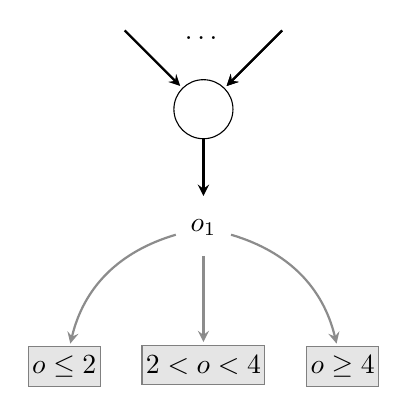
\begin{tikzpicture}
  [->, >=stealth, shorten >=1pt,auto,node distance=2cm,
    align=center,
    neuron/.style={%
      circle, draw, minimum size=0.75cm
    },
    invis/.style={%
      circle
    },
    bucket/.style={%
      rectangle,draw=black!50,fill=black!10,
      minimum size=5mm,inner sep=0.5mm
    },
  ]

  \node[neuron] (o) {};
  \node[invis] (o2) [below of=o, node distance=1.5cm] {$o_1$};

  \draw[->,thick] (o) -- (o2);

  \node[bucket] (b2) [below of=o2, node distance=1.75cm] {$2 < o < 4$};
  \node[bucket] (b1) [below left of=o2, node distance=2.5cm] {$o\leq2$};
  \node[bucket] (b3) [below right of=o2, node distance=2.5cm] {$o\geq4$};

  \draw[->,thick] ++(-1,1) -- (o); 
  \draw[->,thick] ++(1,1) -- (o); 
  \draw[->,thick] ++(1,1) -- (o) node[above=0.75cm] {\dots};

  \path[->,thick,gray,opacity=0.9]
  (o2) edge [bend right] (b1)
       edge (b2)
       edge [bend left] (b3);

\end{tikzpicture}

    \end{figure}
  \end{columns}
\end{frame}
